\documentclass[a4paper,ngerman,12pt]{scrartcl}

\usepackage[utf8]{inputenc}
%\usepackage[ansinew]{inputenc}

\usepackage[ngerman]{babel}

\usepackage{amsmath,amsthm,amssymb,stmaryrd,color,graphicx}
\usepackage{setspace}
\usepackage{bussproofs}
\usepackage{array}
\usepackage{comment}
\usepackage{wrapfig}

\usepackage{enumitem}

\usepackage{units}

\usepackage[protrusion=true,expansion=true]{microtype}

\usepackage{lmodern}

\usepackage{hyperref}
\usepackage{cleveref}

\newcommand{\RR}{\mathbb{R}}
\newcommand{\CC}{\mathbb{C}}
\newcommand{\ZZ}{\mathbb{Z}}
\newcommand{\NN}{\mathbb{N}}
\newcommand{\QQ}{\mathbb{Q}}

\setlength\parskip{\medskipamount}
\setlength\parindent{0pt}

\theoremstyle{definition}
\newtheorem{defn}{Definition}[]
\newtheorem{axiom}[defn]{Axiom}
\newtheorem{bsp}[defn]{Beispiel}

\theoremstyle{plain}
\newtheorem{prop}[defn]{Proposition}
\newtheorem{motto}[defn]{Motto}
\newtheorem{wunder}[defn]{Wunder}
\newtheorem{ueberlegung}[defn]{Überlegung}
\newtheorem{lemma}[defn]{Lemma}
\newtheorem{kor}[defn]{Korollar}
\newtheorem{hilfsaussage}[defn]{Hilfsaussage}
\newtheorem{satz}[defn]{Satz}
\newtheorem{frage}[defn]{Frage}

\theoremstyle{remark}
\newtheorem{bem}[defn]{Bemerkung}
\newtheorem{aufg}[defn]{Aufgabe}

\newtheorem*{antwort}{Antwort}

\newlength{\aufgabenskip}
\setlength{\aufgabenskip}{1.4em}
\newcounter{aufgabennummer}
\newenvironment{aufgabe}[1]{
	\addtocounter{aufgabennummer}{1}
	\textbf{Aufgabe \theaufgabennummer.} \emph{#1} \par
}{\vspace{\aufgabenskip}}

\clubpenalty=10000
\widowpenalty=10000
\displaywidowpenalty=10000

\setlength\unitlength{1cm}

\usepackage{tikz}

\RequirePackage{geometry}
\geometry{textwidth=16.0cm,textheight=24.5cm,footskip=1.5cm}

\begin{document}
	
\begin{picture}(0,0)
\put(0,-0.5){%
	
\includegraphics[scale=0.1]{logo-ifm}
}
\put(14.0,-3.5){%
	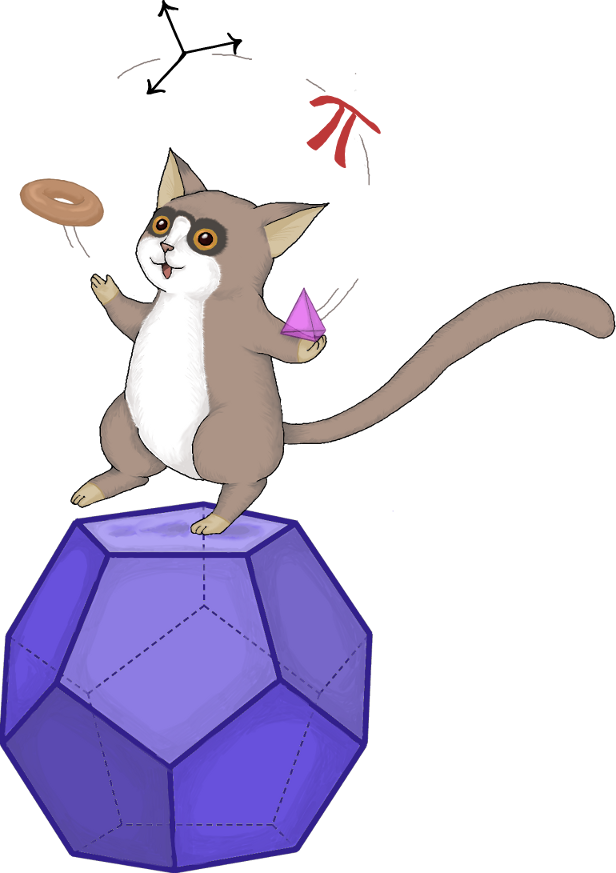
\includegraphics[scale=0.17]{cover}
}
\end{picture} 
	
\vspace{6em}

\section*{Codierungstheorie - Lösungshinweise}

Dieses Skript enthält Lösungs\emph{hinweise} zum letzten Korrespondenzbrief. Manchmal sind dies schon die kompletten Lösungen der Aufgaben, meistens sind es aber nur einige Hinweise, die dir dabei helfen sollen, auch die Aufgaben lösen zu können, bei denen du bisher nicht weiter gekommen bist. Wenn du noch weitere Fragen zu den Aufgaben hast, kannst du uns diese weiterhin gerne per E-Mail stellen.

Wenn du uns bereits deine eigenen Lösungsversuche geschickt hast (oder noch schicken wirst - das ist selbstverständlich immer noch möglich), dann versuchen wir natürlich auch dir mit unseren Korrekturen beim Verständnis der Aufgaben zu helfen. Es lohnt sich also uns deine Lösungen zu senden :-)

\begin{aufgabe}{}
	Die (vermutlich) einfachste Möglichkeit ist es, die Nachricht einfach \emph{dreimal} hintereinander zu schreiben. Sollten dann bei der Übertragung zwei Buchstaben verfälscht werden, so ist immer noch mindestens eine der drei Nachrichten unbeschädigt und der Empfänger kann dadurch erkennen, dass bei der Übertragung Fehler passiert sind.
	
	Tritt bei diesem Verfahren nur ein Fehler auf, so kann dieser sogar korrigiert werden.
\end{aufgabe}

\begin{aufgabe}{}
	Da die Nachricht dreimal hintereinander geschrieben wird, sind die Codewörter also auch dreimal so lang wie die ursprünglichen Nachrichtenwörter. Damit ist die Informationsrate $3$.
\end{aufgabe}

\begin{aufgabe}{}
	172919 ist korrekt, die Nachricht war 1729 (und die Quersumme folglich $1+7+2+9=19$)
	
	422416 ist fehlerhaft, denn wäre die Nachricht $4224$ korrekt, so müssten die letzten beiden Ziffern $4+2+2+4=12$ lauten. Das ursprüngliche Codewort könnte 822416, 462416, 426416, 422816 oder 422412 gelautet haben.
	
	939124 ist ebenfalls fehlerhaft und 314109 ist korrekt (Nachricht 3141).
	
	739150 ist wieder fehlerhaft. Hier kann man aber zusätzlich noch feststellen, dass der Fehler im hinteren Teil passiert sein muss (also in der Prüfsumme), da dieser größer als 36 (der Maximalwert) ist. Falls insgesamt höchstens eine einzige Ziffer verfälscht wurde, muss dies also die Ziffer 5 in der Prüfsumme gewesen sein und die Nachricht selbst ist folglich erhalten geblieben.
\end{aufgabe}

\begin{aufgabe}{}
	23836 ist korrekt, Quersumme ist $2+3+8+3=16$, also Prüfziffer $6$.
	
	99999 ist fehlerhaft, denn die Prüfziffer müsste $6$ sein.
	
	47629 ist korrekt und 38425 falsch.
\end{aufgabe}

\begin{aufgabe}{}
	Die Informationsrate beträgt $\frac{5}{4} = 1,25$.
	
	Die Informationsrate wird besser, wenn man längere Nachrichtenworte verwendet. Verwendet man beispielsweise zehnstellige Ziffern mit einstelliger Prüfsumme, so erhält man eine Informationsrate von $\frac{11}{10} = 1,1$. In der Praxis erhöht sich bei längeren Nachrichtenwörtern aber natürlich auch die Wahrscheinlichkeit, dass mehr als eine einzelne Ziffer verfälscht wird. Eine kleine Informationsrate ist also nicht das einzige Qualitätskriterium eines guten Codierungsverfahrens.
\end{aufgabe}

\begin{aufgabe}{ISBN}
	978-349805241-6 hat abgewandelte Quersumme 110 und ist damit korrekt.
	
	978-357003472-9 hat abgewandelte Quersumme 104 und ist folglich fehlerhaft.
	
	978-184854956-2 hat abgewandelte Quersumme 140 und ist daher wieder korrekt.
\end{aufgabe}

\begin{aufgabe}{}
	Die Informationsrate ist $\frac{13}{12}$
\end{aufgabe}

\begin{aufgabe}{Warum ausgerechnet 3?}
	Multipliziert man die Ziffern von 0 bis 9 mit 2, so erhält man folgende Tabelle
	\begin{center}
		\begin{tabular}{cccccccccc}
			0 & 1 & 2 & 3 & 4 & 5 & 6 & 7 & 8 & 9 \\
			$\downarrow$ & $\downarrow$ & $\downarrow$ & $\downarrow$ & $\downarrow$ & $\downarrow$ & $\downarrow$ & $\downarrow$ & $\downarrow$ & $\downarrow$ \\
			0 & 2 & 4 & 6 & 8 & 10 & 12 & 14 & 16 & 18
		\end{tabular}
	\end{center}
	Wie du siehst, werden hier verschiedene Ziffern auf Zahlen mit der gleichen Einerstelle abgebildet. Bspw. führen damit 1 und 6 zur gleichen Prüfziffer. Ein entsprechender Fehler könnte damit nicht mehr erkannt werden.
	
	Schreibt man sich derartige Tabellen für die anderen einstelligen Zahlen auf, so sieht man, dass 7 und 9 alternative Möglichkeiten zur 3 wären.
\end{aufgabe}

\begin{aufgabe}{Weitere Problempaare}
	Alle Problempaare sind 05, 16, 27, 38 und 49.
	
	Damit die Vertauschung zweier benachbarter Ziffern $x$ und $y$ nicht erkannt wird, muss gelten: 
		\[\text{Einerziffer von }(1\cdot x + 3\cdot y) = \text{ Einerziffer von }(1\cdot y + 3\cdot x)\]
	Diese Gleichung kann man vereinfachen zu 
		\[\text{Einerziffer von }2\cdot y = \text{ Einerziffer von }2\cdot x\]
	Und jetzt kannst du die Tabelle aus Aufgabe 8 verwenden, um alle möglichen Ziffernpaare zu finden, die dies erfüllen.
\end{aufgabe}

\begin{aufgabe}{}
	Korrekt ist nur die dritte Nachricht, bei den ersten beiden muss ein Fehler passiert sein. Korrigiert lauten die Nachrichten:
	\[\begin{array}{ccc}3 & 5 & 8\\1 & 5 & 6 \\ 4 & 0 &\end{array} \quad-\quad \begin{array}{ccc}9 & 9 & 8\\6 & 7 & 3 \\ 5 & 6 &\end{array} \quad-\quad \begin{array}{ccc}4 & 3 & 7\\3 & 8 & 1 \\ 7 & 1 &\end{array}\]
\end{aufgabe}

\begin{aufgabe}{}
	Informationsrate: $\frac{8}{4}=2$
	
	Nachrichtenwörter der Länge 9 kann man in einem $3\times 3$-Quadrat anordnen und dann das gleiche Verfahren anwenden, wie im Brief beschrieben. Dies führt zu einer Informationsrate von $\frac{15}{9}=\frac{5}{3}$.
\end{aufgabe}

\begin{aufgabe}{}
	Passiert ein Fehler im Nachrichtenteil des Codewortes, so werden dadurch immer gleich zwei Prüfziffern falsch (in der entsprechenden Zeile und der entsprechenden Spalte). Passiert der Fehler dagegen bei einer der Prüfziffern selbst, so ist damit insgesamt nur eine einzige Prüfziffer falsch (nämlich die, bei der der Fehler passiert ist). Daran kann der Empfänger also erkennen, dass der Fehler nur im Prüfzifferbereich passiert ist und die Nachricht daher unverfälscht sein muss.
\end{aufgabe}

\end{document}